\begin{figure}[htbp]
\centering
\adjustbox{valign=t}{
   \begin{tabular}{p{6cm}c}
        \toprule
         \v~$= \begin{pmatrix}
             0 & 0 & 4 & 3
         \end{pmatrix}$ with branch lengths represented in two rows $\bm{\beta_1}$ and $\bm{\beta_2}$ & \adjustbox{valign=t}{
         \m~=~
         $\left(\begin{array}{c|cccc}
         \bm{v} & 0 & 0 & 4 & 3 \\
         \bm{\beta}_1 & a_1 & b_1 & c_1 & d_1 \\
         \bm{\beta}_2 & a_2 & b_2 & c_2 & d_2 \\
        \end{array}\right)$
        } \\
        \midrule
        Branch lengths are attributed to edges using the ancestry matrix \\ BL(3, 5) = $a_1$ \newline BL(4, 5) = $a_2$ \newline ... \newline BL(7, 8) = $d_1$ \newline BL(5, 8) = $d_2$ & \adjustbox{valign=t}{
        $\bm{a} = \begin{bmatrix}
        \rn{c11}{3} & \rn{c12}{4} & \rn{p1}{5} & \rn{a1}{a_1} & \rn{a2}{a_2} \\
        0 & 2 & 6 & b_1 & b_2 \\
        6 & 1 & 7 & c_1 & c_2 \\
        \rn{c31}{7} & \rn{c32}{5} & \rn{p3}{8} & \rn{c1}{d_1} & \rn{c2}{d_2} \\
        \end{bmatrix}$}
        \begin{tikzpicture}[overlay,remember picture]
            \path[every node/.style={font=\sffamily\small}]
                (c11) edge[bend right, red] node [left] {} (a1)
                (p1) edge[bend right, red] node [left] {} (a1)
                (c12) edge[bend left, blue] node [left] {} (a2)
                (p1) edge[bend left, blue] node [left] {} (a2)
                (c31) edge[bend left, red] node [left] {} (c1)
                (p3) edge[bend left, red] node [left] {} (c1)
                (c32) edge[bend right, blue] node [left] {} (c2)
                (p3) edge[bend right, blue] node [left] {} (c2);
        \end{tikzpicture} \\
        \midrule
        Annotated tree & \adjustbox{valign=t}{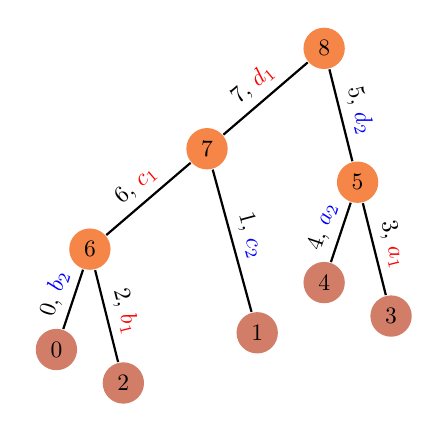
\begin{tikzpicture}[thick, scale=0.85, every node/.style={scale=0.85}]
            \node[circle, fill=Mahogany!50] (0) at (0, -0.5) {0};
            \node[circle, fill=Mahogany!50] (1) at (3, -0.25) {1};
            \node[circle, fill=Mahogany!50] (2) at (1, -1) {2};
            \node[circle, fill=Mahogany!50] (3) at (5, 0) {3};
            \node[circle, fill=Mahogany!50] (4) at (4, 0.5) {4};
            \node[circle, fill=Peach] (5) at (4.5, 2) {5};
            \node[circle, fill=Peach] (6) at (0.5, 1) {6};
            \node[circle, fill=Peach] (7) at (2.25, 2.5) {7};
            \node[circle, fill=Peach] (8) at (4, 4) {8};

            \draw (8) -- node[midway, sloped, above] {{5, \textcolor{blue}{$d_2$}}} (5);
            \draw (8) -- node[midway, sloped, above] {{7, \textcolor{red}{$d_1$}}} (7);
            \draw (7) -- node[midway, sloped, above] {{6, \textcolor{red}{$c_1$}}} (6);
            \draw (6) -- node[midway, above, sloped] {{2, \textcolor{red}{$b_1$}}} (2);
            \draw (7) -- node[midway, sloped, above] {{1, \textcolor{blue}{$c_2$}}} (1);
            \draw (6) -- node[midway, sloped, above] {{0, \textcolor{blue}{$b_2$}}} (0);
            \draw (5) -- node[midway, sloped, above] {{3, \textcolor{red}{$a_1$}}} (3);
            \draw (5) -- node[midway, sloped, above] {{4, \textcolor{blue}{$a_2$}}} (4);
        \end{tikzpicture}}\\
        \bottomrule
    \end{tabular}
}
\caption{Visual representation of an extended version of the phylo2vec vector with branch lengths, using \v~$= \begin{pmatrix}
    0 & 0 & 4 & 3
\end{pmatrix}$ as an example. Adapted from Scheidwasser \textit{et al.}~\cite{scheidwasser2025}.}
\label{fig:phylo2mat}
\end{figure}